%%%% Various options for document class.
\documentclass[usenatbib, a4paper]{mn2e}
%%\documentclass[preprint2, a4paper, 11pt]{aastex}
%%\documentclass[twocolum]{revtex4}
%%\documentclass{report}
% \documentclass[useAMS,usenatbib,referee]{mn2e}

%\usepackage{psfig,morefloats,url}
%use preprint2 for 2 columns paper.

%% declare any packages used
\usepackage{graphicx}
\usepackage{natbib}
\usepackage{graphicx}
\usepackage{color}
\usepackage{pdfpages}
\usepackage{appendix}
%\usepackage{epsfig}
%\usepackage[dvips]{color}
%\usepackage{aabib}


%\marginparwidth = 25pt
\citestyle{aa}
\addtolength{\topmargin}{-.5in}
%% This command added as margins are wrong in mn2e, it appears. 
%% Not needed for other classes




%%%%%%%%%%%%%%%%%%%%%%%%%%%%%%%%%%%%%%

\begin{document}
%% define bibstyle and other definitions
\bibliographystyle{aabib}
%% renew commands
\renewcommand{\labelitemi}{$-$}
\def\la{Ly-$\alpha$ }
\def\py{\textsc{Python} }
\def\civ{C~\textsc{iv} }
\def\araa{ARAA}
\def\nat{Nature}
\def\apjl{ApJ Letters}
\def\aapr{AAPR}
\def\ssr{SSR}
\def\apj{ApJ}
\def\pasp{PASP}
\def\aap{A\&A}
\def\mnras{MNRAS}
\def\aj{AJ}
\def\rmxaa{RMXAA}

%%%%%%%%%%%%%%%%%%%%%%%%%%%%%%%%%%%%%%
%
%          TITLE AND AUTHORS
%
%%%%%%%%%%%%%%%%%%%%%%%%%%%%%%%%%%%%%%%

\title[Optical Lines from CV Disk Winds]
{The Disk Wind Contribution to Optical Lines in Cataclysmic Variables}

\author[Matthews et al.]{J.~H.~Matthews$^1$\thanks{jm8g08@soton.ac.uk},C.~Knigge,$^1$ K.~S.~Long,$^2$ S.~A.~Sim,$^3$ and N.~Higginbottom$^1$
\medskip  
\\$^1$School of Physics and Astronomy, University of Southampton, Highfield, Southampton, SO17 1BJ, United Kingdom
\\$^2$Space Telescope Science Institute, 3700 San Martin Drive, Baltimore, MD, 21218
\\$^3$School of Mathematics and Physics, Queens University Belfast, University Road, Belfast, BT7 1NN, Northern Ireland, UK}

\date{\today}


%%%%%%%%%%%%%%%%%%%%%%%%%%%%%%%%%%%%%%
%
%          ABSTRACT
%
%%%%%%%%%%%%%%%%%%%%%%%%%%%%%%%%%%%%%%%
\maketitle

%% This is the end of the preamble.  Indicate the beginning of the
%% paper itself with \begin{document}.




\begin{abstract}
Disk-dominated High-State Cataclysmic Variable systems (CVs) exhibit strong emission in optical recombination lines.
Here we present results obtained by improving a Monte Carlo radiative transfer code originally used
to model UV resonance lines in CVs, which show the potential contribution to these optical lines
from a line driven accretion disk wind.
\end{abstract}


\begin{keywords}
Cataclysmic Variables - quasars: absorption lines - radiative transfer - 
methods: numerical.
\end{keywords}

%%%%%%%%%%%%%%%%%%%%%%%%%%%%%%%%%%%%%%
%
%          INTRODUCTION
%
%%%%%%%%%%%%%%%%%%%%%%%%%%%%%%%%%%%%%%%

\section{Introduction} 

Cataclysmic Variables (CVs), are systems in which a white dwarf accretes matter from a donor star
via Roche-lobe overflow. In Disk-dominated CVs, this accretion is mediated by an accretion disk which forms 
around the white dwarf, and it has been shown that the spectra of high state CVs
exhibit absorption features believed to be caused by an outflow, potentially line-drive,
rising from the accretion disk. 

The ultraviolet spectra of CVs, in particular, exhibity P-Cygni like profiles in resonance lines such as 
NV, OVI and, most commonly, CIV.




%%%%%%%%%%%%%%%%%%%%%%%%%%%%%%%%%%%%%%
%
%          CODE
%
%%%%%%%%%%%%%%%%%%%%%%%%%%%%%%%%%%%%%%%

\section{Description of the code}

\py is a Monte Carlo radiative transfer code which uses the Sobolev approximation. It is originally
introduced by Long \& Knigge (2002), and a more up-to-date description is provided by
Higginbottom et al. (2013). 


\subsection{Macro-atoms}
In its standard operating mode, \py uses a two-level atom approximation (see e.g Mihalas 1982\nocite{mihalas}, Ch. 11) for its treatment of lines. This approximation works well when treating so-called `resonance lines' (such as \civ, O\textsc{vi}), in which the excited electron is strongly coupled to the ground state, but breaks down for more complex situations such as recombination cascades. To properly model recombination lines, including the Lyman and Balmer series, a more complete treatment of line transfer is required.

Lucy (2002, 2003\nocite{lucy2002, lucy2003}; hereafter L02, L03) showed that by quantising matter into `macro-atoms', and radiant and kinetic energy into energy packets, it is possible to asymptotically reproduce the emisssivity of a gas in statistical equilibrium without simplifying line transfer. Macro-atoms are finite volume elements with internal transition probabilities that are `activated' by packets of radiant (r-packets) or kinetic (k-packets) energy. A typical activation and deactivation sequence is shown in figure~\ref{macro}.
A full description is far beyond the scope of this report- consult L02 and L03. 

The macro-atom scheme has been used with \py before, in a Hydrogen-only mode with application to YSOs \citep{simmacro2005}, but has not yet been applied to AGN or CV problems. With some improvements, the current scheme will enable \py to model H and He recombination lines, for example. The fast, simple treatment of resonance lines 
can be retained, as the \py implementation allows for non-macro atom treatment for certain ions.




%%%%%%%%%%%%%%%%%%%%%%%%%%%%%%%%%%%%%%
%
%          MATOM TESTING
%
%%%%%%%%%%%%%%%%%%%%%%%%%%%%%%%%%%%%%%%

\section{Testing the macro atom scheme}

Before proceeding with modeling of CV systems, we need to be sure that our scheme fulfils Lucy's (2002) 
statement that it will `asymptotically reproduce the emissivity of a gas in statistical equilibrium'.
For our tests, we use a Hydrogen only `thin shell' mode in \py, in which a single macro atom is created as a spherical 
shell with a thickness of 1cm. We construct the situation such that all opacities other than 
bound-free absorption are negligible, and the only cooling process available to the gas is that of
recombination line emission. This is a mathematical pathology, commonly known as `Case A', and allows
us to test against analytical calculations.

As \py normally models dense environments, it assumes each principal quantum number level is
well `l-mixed' - that is each subshell of a given level is populated according to statistical weight by
inelastic collisions. It is therefore not possible to compare with non-L mixed calculations such as 
those presented in Osterbrock (1989\nocite{oster}). Seaton (1959; S59\nocite{seaton}) carried out calculations
for Case A in the l-mixed case, and is thus a better comparison. Figure 1 shows a comparison between S59
and \py, showing excellent agreement. Figure 2 shows the Case B comparison, in which the escape probabilities
for the Lyman lines have been explicitly zeroed.

\begin{figure}
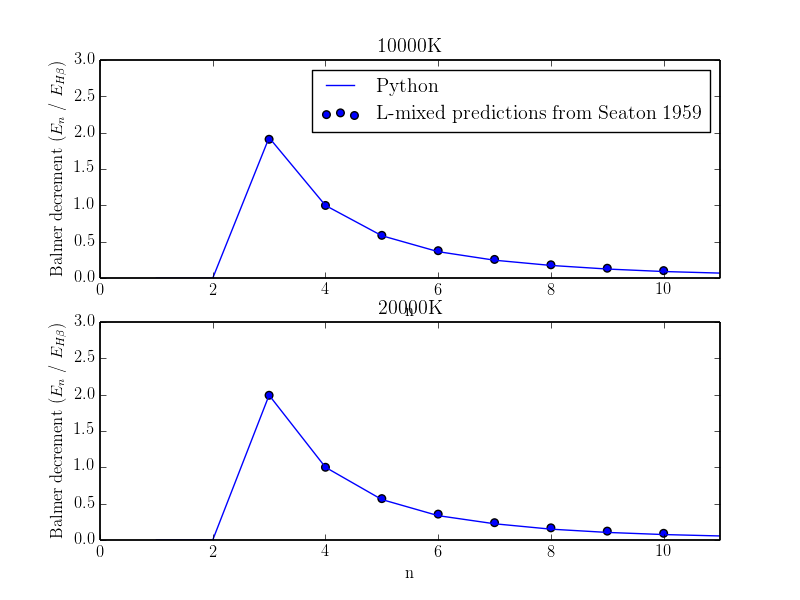
\includegraphics[width=0.5\textwidth]{caseA.png}
\caption{Case A comparison between S59 and \py at 10000K and 20000K}
\end{figure}

\begin{figure}
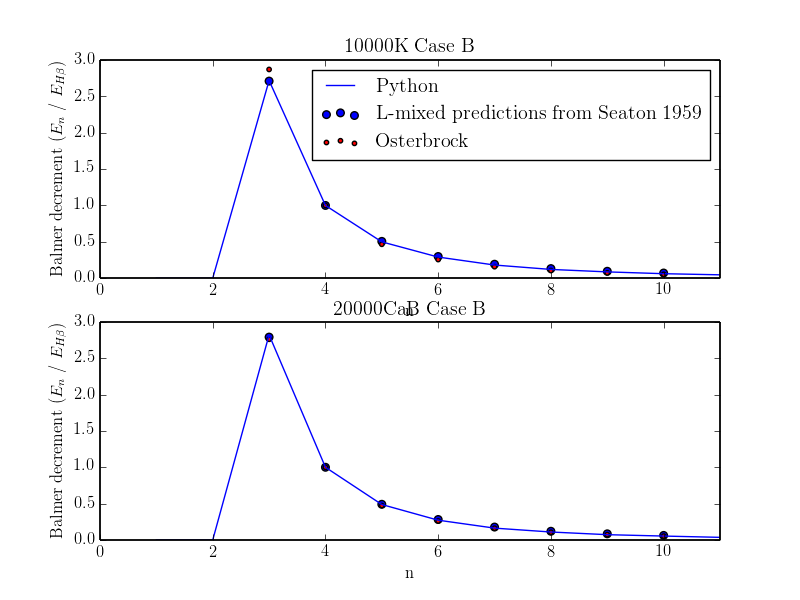
\includegraphics[width=0.5\textwidth]{caseB.png}
\caption{Case B comparison between S59 and \py at 10000K and 20000K}
\end{figure}

This test verifies the treatment of recombination lines in Hydrogen only models, but it is also necessary to test the implementation
of macro-atoms when other elements are treated as so-called `simple ions'. In this mode, the user can select which species to treat as
macro atoms, meaning that the other species are still treated with a two-level approximation. This means that the fast treatment of
resonance lines can be maintained without sacrificing the necessity that all energy packets are indivisible. It is important to verify that 
this still produces the correct ionization state for the wind. We can test this by comparing against both {\textsc Cloudy} and LK02.



%%%%%%%%%%%%%%%%%%%%%%%%%%%%%%%%%%%%%%
%
%          MATOM TESTING
%
%%%%%%%%%%%%%%%%%%%%%%%%%%%%%%%%%%%%%%%

\section{The CV Model}
As in LK02, we follow the prescription of SV93 in both our fundamental biconical wind model and velocity law


%%%%%%%%%%%%%%%%%%%%%%%%%%%%%%%%%%%%%%
%
%          RESULTS
%
%%%%%%%%%%%%%%%%%%%%%%%%%%%%%%%%%%%%%%%

\section{Results from Simulations}


%%%%%%%%%%%%%%%%%%%%%%%%%%%%%%%%%%%%%%
%
%          DISCUSSION
%
%%%%%%%%%%%%%%%%%%%%%%%%%%%%%%%%%%%%%%%


\section{Discussion}

%% Balmer jump


\subsection{Future Work}

In addition to this project, we plan to apply the macro atom scheme to QSOs in order to build on the work of Higginbottom et al. (2013),
in which a benchmark biconical disk wind model was presented. In particular, we hope that the macro-atom scheme will enable the
model to produce significant Lyman-$\alpha$ emission, as is observed in QSOs.




\bibliography{mybib.bib}

\end{document}
